\documentclass{article}
\usepackage{algorithm}
\usepackage{algpseudocode}
\usepackage{graphicx}
\title{CSEP521 : Applied Algorithms: Homework 1}
\author{Karuna Sagar Krishna}
\begin{document}
\maketitle

\section*{Question 1}
The functions in increasing order of asymptotic growth rate is - \[ f6, f4, f1, f2, f3, f5 \]

\section*{Question 2}

\subsection*{Idea}
As hinted in the question, entries in \(A^k\) is the number of walks of length \(k\). So, we compute \(A^k\) using exponentiation by squaring method. With this, we can count all the walks of length \(k\) in graph G, by adding the values of \(A^k[i][j]\). Note, for undirected graph due to its symmetry we will be double counting and hence we half the count before returning.

\subsection*{Algorithm}
\begin{algorithm}
/* Assume procedure $MatrixMultiple(A, B)$ is given that runs in $O(n^\omega)$ */
\begin{algorithmic}
\Procedure{Exponential}{$A, k$}
    \If {$k = 0$}
        \State \textbf{return 1}
    \EndIf
    \If {$k = even$}
        \State \textbf{return} $Exponential(MatrixMultiple(A, A), k/2)$
    \EndIf
    \If {$k = odd$}
        \State \textbf{return} $MatrixMultiple(A, Exponential(MatrixMultiple(A, A), (k-1)/2))$
    \EndIf
\EndProcedure
\end{algorithmic}
\end{algorithm}

\begin{algorithm}
\begin{algorithmic}
\Procedure{CountWalk}{$A, k$}
    \State $Ak = Exponential(A, k)$
    \State $c = 0$
    \For {$i \in 0 \dots n$}
        \For {$j \in 0 \dots n$}
            \State $c += A[i][j]$
        \EndFor
    \EndFor
    \State \textbf{return} c/2\Comment{for directed graph return c}
\EndProcedure
\end{algorithmic}
\end{algorithm}

\subsection*{Correctness}
Consider adjacency matrix $A$ representing graph G, where \(A[i][j] \in \{0, 1\}\). Lets prove that \(A^k[i][j]\) is equal to the number of walks of length k that start at \(i\) and end at \(j\).

When \(k = 0\), it is clear that the above claims holds true. $A[i][j]$ indicates the number of walks of length 1 between vertex $i$ and $j$. Note, this is the same as the definition of adjacency matrix.

By induction, assume that this claim holds good for some \(k > 0\). Matrix \(A^{k+1}\) can be computed as \(A^k*A\). Lets denote \(A^k\) as \(B\). By matrix multiplication definition, we compute \(A^{k+1}[i][j])\) entry as \(\sum(B[i][l]*A[l][j])\) for all \(l\). Note, \(B[i][j]\) indicates the number of walks of length \(k\) while \(A[i][j]\) indicates the number of walks of length \(1\). So, for some \(l\), \(B[i][l]*A[l][j]\) indicates the number of walks from \(i\) to \(j\) of length \(k+1\) passing through $l$ i.e. number of walks of length \(k\) from \(i\) to \(l\) and then following one edge from \(l\) to \(j\). Hence, \(A^{k+1}[i][j] = \sum(B[i][l]*A[l][j])\) for all \(l\), indicates the sum of all walks of length \(k+1\) from \(i\) to \(j\)

So, to get the count of all walks of length \(k\) in graph G, we sum the values of \(A^{k+1}[i][j])\) for all \(i\) and \(j\). In case of undirected graph \(A[i][j] = A[j][i]\) since they represent the same edge in G. Hence, we address this by halving the sum. This is not required for directed graphs, since edge \(A[i][j]\) and \(A[j][i]\) represent different edges in G.

\subsection*{Analysis}
The \(Exponential\) procedure involves \(\log k\) matrix multiplications. The matrix multiplication algorithm is assumed to be given with a running time of \(O(n^\omega)\). Hence \(Exponential\) procedure requires \(O(n^\omega \log k)\).

The \(CountWalk\) procedure iterates through the entire matrix having \(n^2\) entries hence has a runtime of \(O(n^2) + O(n^\omega \log k) = O(n^\omega \log k)\) since \(\omega >= 2\)

\section*{Question 3}

\subsection*{Question 3a}

\subsection*{Idea}
A complete graph is a graph where there is an edge between every pair of vertices. In such a graph, each vertex has a degree of \(n-1\) and this is the maximum degree. The claim is that we can be able to color this complete graph with \((n-1)+1 = n\) colors. It is obvious that such a coloring is possible since we have a distinct color for each vertex of the graph. So the claim holds in complete graph. And it seems unlikely to come up with a counter example to the claim.

Consider a vertex of graph $G$, its degree is equal to or less than $\Delta$ (maximum degree of $G$). We have $\Delta+1$ available colors. So by pigeon hole principle, it is must be possible to assign colors to all vertices in $G$

\subsection*{Algorithm}
\begin{algorithm}
\begin{algorithmic}
\Procedure{DeltaPlusOneColoring}{$A$}
    \State $availableColors = \{0..\Delta\}$ for each vertex
    \State $vertexColor = NULL$ for each vertex
    \For {$i \in 0 \dots n$}
        \If {$vertexColor[i] != NULL$}
            \State /* Need this check for 3b where the graph is partially colored */
            \State \textbf{continue}
        \EndIf
        \State $vertexColor[i] = $ first color in $availableColors[i]$
        \For {$j \in 0 \dots n$}
            \If {$A[i][j] = 1 \land vertexColor[j] = NULL$}
                \State $availableColors[j] = availableColors[j] - \{vertexColor[i]\}$
            \EndIf
        \EndFor
    \EndFor
\EndProcedure
\end{algorithmic}
\end{algorithm}

\subsection*{Correctness}
Proving the claim by induction. For base case, $n=1$ the maximum degree is 0 since there cannot be any edge in a graph with only one vertex. Hence the algorithm colors this with 1 color i.e. maximum degree + 1.

Consider a graph with $n$ nodes. Lets consider some vertex $v$, if we remove this node and all the corresponding edge we are left with a subgraph with $n-1$ nodes and maximum degree of $\Delta^\prime <= \Delta$. This subgraph by induction can be colored with $\Delta^\prime+1$ colors. If $\Delta^\prime = \Delta$, then $v$ has atmost $\Delta$ colored neighbors and we have one available color to paint $v$. If $\Delta^\prime < \Delta$, then $v$ has $\Delta$ colored neighbors and we have one available color to paint $v$. Hence, we can color this graph with $\Delta+1$ colors.

The algorithm maintains the invariant that $vertexColor$ for any vertex is either NULL or has a color that doesn't conflict with its neighbors. Suppose this was not the case, it would imply that when $v$ was assigned a color $c$ from $availableColors[v]$ which is used to color one of its neighbor $u$. This cannot happen since when the neighbor $u$ was colored with $c$, we removed this color from $availableColors[v]$ since $A[u][v]$ are neighbors and $v$ was not assigned a color.

Suppose the algorithm runs out of colors i.e. $availableColors[v] = \emptyset$ when the outer loop $i=v$. This implies that all $\Delta+1$ colors were removed from $availableColors[v]$. For this to happen, we must have had $\Delta+1$ neighbors who have take up all the available colors. This contradicts since the  degree of $v <= \Delta$. So the algorithm can always find a valid coloring for a vertex.

Putting these together, we see that the algorithm can color the entire graph correctly with $\Delta+1$ colors.

\subsection*{Analysis}
The algorithm terminates after a maximum of $O(n^2)$ steps since there are 2 nested loops. We can improve this nested loop further by using an adjacency list representation of the graph leading to $O(n+m)$ runtime since we need to visit every vertex and all the edges once.

\subsection*{Question 3b}

\subsection*{Idea}
Since graph $G$ is promised to have 3-coloring, it follows that we can color any subgraph with 3 colors. Suppose that is not true i.e. there is a subgraph $G^\prime$ that cannot be 3 colored and requires 4 or more colors. If so, $G$ would also require 4 or more colors since all the edges and vertices of $G^\prime$ are part of $G$. This violates the promise of having $G$ 3 colorable, hence a contradiction. So $G^\prime$ can be 3 colored.

The rest of the idea is to follow steps provided by the hint associated with the question.

\subsection*{Algorithm}
\begin{algorithm}
\begin{algorithmic}

\State $vertexColor = NULL$ for each vertex
\State $degree = $ degree of each vertex
\State $currentColor = 0$

\Procedure{ThreeColorSubgraph}{$A, i$}
    \State $vertexColor[i] = currentColor$
    \State Use currentColor+1 and currentColor+2 to color neighbors of i using BFS
    \State $currentColor += 3$
\EndProcedure

\Procedure{SqrtNColoring}{$A$}
    \For {$i \in 0 \dots n$}
        \If {$vertexColor[i] = NULL \land degree[i] >= \sqrt n$}
            \State $ThreeColorSubgraph(A, i)$
        \EndIf
    \EndFor

    \State /*Color the rest using new colors starting with $currentColor$ and above*/
    \State $DeltaPlusOneColoring(A)$
\EndProcedure
\end{algorithmic}
\end{algorithm}

\subsection*{Correctness}
$ThreeColorSubgraph(A, i)$ colors a subgraph of $G$ i.e. subgraph containing $i \cup neighbors(i)$. This subgraph is 3 colorable as proved above. This is achieved in a straightforward manner by coloring $i$ with first new color and its neighbors with next 2 new colors. In other words, the $neighbors(i)$ form a bipartite graph. As hinted and seen in class, this bipartite graph can be colored using BFS algorithm where all vertices in same BFS layer gets the same color. Note, BFS is run on the subgraph formed by $neighbors(i)$. Also, note that we are not reusing colors across $ThreeColorSubgraph(A, i)$ invocation, so we need $3k$ colors where $k$ is the number of vertices with degree larger than $\sqrt n$.

We have already shown that $DeltaPlusOneColoring(A)$ is correct in the previous section. One difference from previous section is that this algorithm is invoked with a partially colored graph. This difference does not impact the correctness or the analysis of this algorithm since we are not reusing the colors from $ThreeColorSubgraph(A, i)$. So we require $\sqrt n+1$ new colors to color the remaining vertices of $G$.

Notice, each invocation of $ThreeColorSubgraph(A, i)$ colors atleast $\sqrt n + 1$ vertices i.e. vertex $i$ and its neighbors, which are atleast $\sqrt n$. So, before $DeltaPlusOneColoring(A)$ is invoked, we have colored atleast $k(\sqrt n + 1)$. This must be less than the $n$ i.e. $k(\sqrt n + 1) <= n \equiv k\sqrt n <= n \equiv k <= \sqrt n$. And in total, we need $3k + \sqrt n + 1$ i.e. atmost $3\sqrt n + \sqrt n + 1 = 4\sqrt n$ colors. In other words, $O(\sqrt n)$ colors are required to color $G$.

\subsection*{Analysis}
$ThreeColorSubgraph(A, i)$ assigns new colors to vertex $i$ and its neighbors using BFS that is run on the subgraph of $neighbors(i)$. And this procedure can potentially be invoked for every vertex of the graph taking a total of $O(n+m)$ steps. As we've seen in the previous section, $DeltaPlusOneColoring(A)$ takes $O(n+m)$ steps as well. So overall, $SqrtNColoring(A)$ takes $O(n+m)$ steps.

\section*{Question 4}

\begin{center}
\begin{tabular}{|c|c|c|}
\hline
dst vertex & length & prev vertex \\
\hline
s & 0 & s \\
\hline
a & 0 & b \\
\hline
b & 3 & e \\
\hline
c & 4 & a \\
\hline
d & -3 & b \\
\hline
e & 0 & h \\
\hline
f & 2 & s \\
\hline
g & 4 & s \\
\hline
h & -2 & i \\
\hline
i & 0 & j \\
\hline
j & 4 & f \\
\hline
\end{tabular}
\end{center}

\begin{figure}[!htb]
    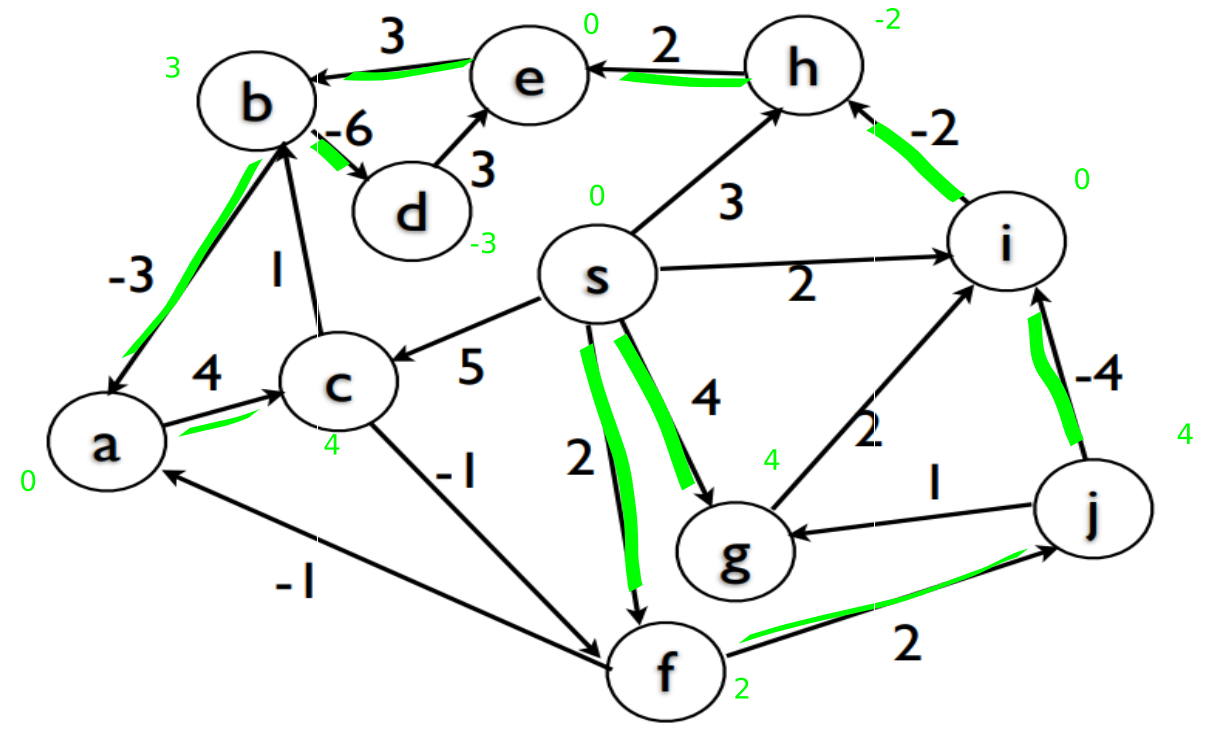
\includegraphics[width=1\textwidth]{shortestPathTree.png}
\end{figure}

\end{document}